\documentclass[letter,10pt]{article}
\usepackage{authblk}
\usepackage{geometry}
\geometry{margin=0.5in}
\usepackage{graphicx}
\graphicspath{ {./images/} }
\usepackage{enumitem}
\usepackage{amsmath}
\usepackage{amssymb}
%\usepackage{biblatex}
\usepackage[backend=biber]{biblatex}
\addbibresource{references.bib}

\begin{document}
\title{An Introduction to and Analysis of the Hollow Heap Data Structure with a Comparison to the Fibonacci Heap Data Structure}
\author{Alisha Sprinkle and Courtney Dixon}
%\affil{CS 5110 - The Design and Analysis of Algorithms}
\date{December 8, 2019}
\maketitle

\section{Abstract}
``For the paper, I would like you to explain the data structure clearly and the amortized analysis. Try to use the accounting method as sometimes that is easier to visualize what is happening in the operations. For the extension, you may implement this data structure, then implement Fibonacci heaps and compare the two in terms of practical efficiency."

\section{Introduction}
Little bit of this and that talk

\section{Hollow Heap: the data structure}
``Clearly explain the data structure"

\section{Analysis}
``Amortized Analysis via Accounting Method"

\section{Hollow Heap Implementation} 
\subsection{Methods}
%\begin{enumerate}
%\begin{enumerate}[label=(\alph*)]
%\renewcommand{\labelitemi}{$\blacksquare$}
\renewcommand\labelitemi{$\square$}
\begin{itemize}
    \item \quad makeHeap()
    \item \quad insert(HollowNode e, int key, HollowHeap h)
    \item \quad meld(HollowHeap g, HollowHeap h)
    \item \quad findMin(HollowHeap h)
    \item \quad decreaseKey(HollowNode e, int key, HollowHeap h)
    \item \quad deleteMin(HollowHeap h)
    \item \quad delete(HollowNode e, HollowHeap h)
    \item \quad doRankedLinks(HollowNode u)
    \item \quad doUnrankedLinks()
    \item \quad makeNode(HollowNode e, int key)
    \item \quad link(HollowNode v, HollowNode w)
    \item \quad addChild(HollowNode v, HollowNode w)
\end{itemize}
%\end{enumerate}
%\end{enumerate}[label=(\alph*)]
\subsection{Pictures}
\begin{center}
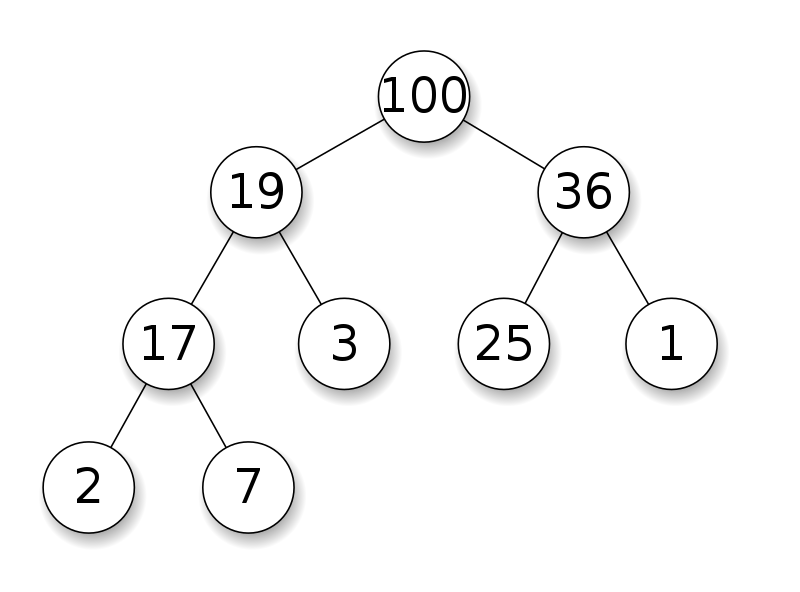
\includegraphics[scale=.5]{Max-Heap.png}
\end{center}
%\begin{center}
%\includegraphics{.png}
%\end{center}

\section{Fibonacci Heap Implementation} 
\subsection{Methods}
%\begin{enumerate}
%\begin{enumerate}[label=(\alph*)]
%\renewcommand{\labelitemi}{$\blacksquare$}
\renewcommand\labelitemi{$\square$}
\begin{itemize}
    \item \quad FibonacciHeap()
    \item \quad insert(Node newNode)
    \item \quad cut(Node cutNode, Node fromNode)
    \item \quad cascadeCut(Node cutNode)
    \item \quad makeChild(Node child, Node parent)
    \item \quad decreaseKey(Node decNode, int ket)
    \item \quad findMin()
    \item \quad delete(Node dNode)
    \item \quad consolidate()
    \item \quad displayHeap()
\end{itemize}
\subsection{Pictures}
%\begin{center}
%\includegraphics[scale=.5]{.png}
%\end{center}
%\begin{center}
%\includegraphics{.png}
%\end{center}

\section{Hollow versus Fibonacci: a comparison}
``Compare the two data structures in terms of practical efficiency"
\subsection{Similarities}
\begin{enumerate}
    \item 
    \item
    \item
\end{enumerate}

\subsection{Dissimilarities}
\begin{enumerate}
    \item 
    \item 
    \item 
\end{enumerate}




\newpage
\nocite{*}
\printbibliography

\end{document}

